\chapter{Different control strategies}

\section{Manoeuvring the vessel using the LOS method}
Path-following problems for vessels are often solved by implementing \ac{LOS} algorithms. Opposite to other position control algorithms, where the vessel may be driven both in longitudinal and transversal directions to converge to a path, the \ac{LOS} algorithm gives a more natural motion towards the desired path. This is done by giving a more natural reference to the heading of the vessel. One of the advantages of this is that it can be applied both to fully actuated and under actuated vessels.

Since it is only the leader, and not any of the followers, who need to follow a path, this is only applied on one vessel. This can also be extended to a leader in a virtual structure. To apply the \ac{LOS} algorithm a setup is needed. To get an overview of the functionality of the \ac{LOS} algorithm see figure~\vref{fig:allinallframes}.
\begin{figure}[htbp]
	\centering
	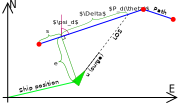
\includegraphics[width=\textwidth]{fig/allinallframes}
	\caption{A ship placed beside the path and uses the \ac{LOS} algorithm to get back on track.}
	\label{fig:allinallframes}
\end{figure}